
\documentclass[hyperref={colorlinks,citecolor=blue,linkcolor=blue,urlcolor=blue}]{beamer}

% For more themes, color themes and font themes, see:
% http://deic.uab.es/~iblanes/beamer_gallery/index_by_theme.html
%
\hypersetup{hidelinks}

\mode<presentation>
{
	\usetheme{Madrid}       % or try default, Darmstadt, Warsaw, ...
	\usecolortheme{default} % or try albatross, beaver, crane, ...
	\usefonttheme{serif}    % or try default, structurebold, ...
	\setbeamertemplate{navigation symbols}{}
	\setbeamertemplate{caption}[numbered]
	\setbeamercolor{title in head/foot}{parent=subsection in head/foot}
} 

\usepackage[bulgarian]{babel}
\usepackage[utf8x]{inputenc}
\usepackage{chemfig}
\usepackage[version=3]{mhchem}
\usepackage{pgfpages}


% Here's where the presentation starts, with the info for the title slide
\title[ ]{Оптични ефекти в изкривено пространство-време: лещи, сенки и поляризация на светлина}
\author[В. Делийски]{Докторант Валентин Делийски}
\institute[Теоретична Физика]{Катедра Теоретична Физика, Физически факултет, СУ "св. Климент Охридски"}
\date{\today}


\begin{document}
	
	\begin{frame}
		\titlepage
		\centering	
		
\includegraphics[scale = 0.5]{Pre-Defence/logo-FzF.png}
	\end{frame}
	
	% These three lines create an automatically generated table of contents.
	\begin{frame}{Outline}
		\tableofcontents
	\end{frame}
	
	\section{Предмет на дисертацията}
	
	\begin{frame}{Радио наблюдения на свръхмасивни компактни обекти}
		
		\centering
		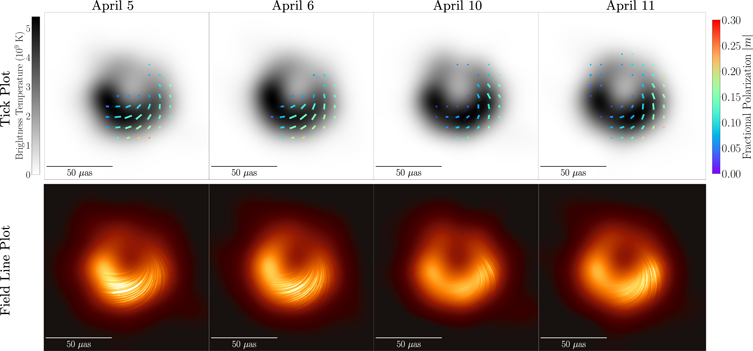
\includegraphics[scale = 0.4]{Pre-Defence/EHT_M87_pol.jpg}\\
		
		\tiny The Event Horizon Telescope Collaboration et al 2021 ApJL 910 L12
		
	\end{frame}
	
	\subsection{Отпечатъкът на пространство-времето върху радио наблюдения на свръхмасивни компактни обекти}
	
	\begin{frame}{Моделиране на М$87^*$ като екзотичен компактен обект}		
		
		\begin{block}{Допускаме следната хипотеза:}
			Наблюденията на EHT могат да
			бъдат възпроизведени от синхотронно излъчваща плазма, около свръхмасивни
			компактни обекти които \textbf{не} притежават хоризонт на събитията.
		\end{block}	
		
		\begin{center}
			$\downarrow$
		\end{center}
		\begin{alertblock}{Задаваме следният въпрос:}
			По какъв начин природата на пространство-времето се отпечатва върху получените чрез радио наблюдения образи?
		\end{alertblock}
		\begin{center}
			$\downarrow$
		\end{center}
		\begin{block}{Сравнителен анализ}
			Моделираме М87$^*$ като екзотичен компактен обект и симулираме неговите радио наблюдения.
		\end{block}
		
	\end{frame}
	
	\subsection{Публикации}
	
	\begin{frame}{Характеристики на наблюдаваните образи}
		\begin{block}{Природата на пространство-времето може (най-общо казано) да повлияе върху следните свойства на получените образи:}
			\centering
			$\bullet$ Морфологията\\
			$\bullet$ Поляризацията
			\begin{alertblock}{$ $}
				\centering
				$\bullet$ Променливостта
			\end{alertblock}
			
		\end{block}
		
		Променливостта, която за Sgr A$^*$ е значителна, се очаква да се влияе предимно от спецификите на акреционният поток, поради което \textbf{не} я разглеждаме в дисертацията.
		
	\end{frame}
	
	\begin{frame}{Публикации}
		
		\begin{block}{Публикации, разглеждащи морфологията}
			$\bullet$ V Deliyski, G Gyulchev, P Nedkova, and S Yazadjiev. Observational features
			of thin accretion disks around traversable wormholes. Journal of Physics:
			Conference Series, 2255(1):012002, apr 2022.\\
			$\bullet$ V Deliyski, G Gyulchev, P Nedkova, and S Yazadjiev.
			Observing naked singularities by the present and next-generation event horizon
			telescope. http://arxiv.org/abs/2401.14092, 2024.
		\end{block}
		
		\begin{block}{Публикации, разглеждащи поляризацията}
			$\bullet$ V Deliyski, G Gyulchev, P Nedkova, and S Yazadjiev.
			Polarized image of equatorial emission in horizonless spacetimes: Traversable
			wormholes. Phys. Rev. D, 106:104024, Nov 2022.\\
			$\bullet$ V Deliyski, G Gyulchev, P Nedkova, and S Yazadjiev.
			Polarized image of equatorial emission in horizonless spacetimes: Naked
			singularities. Phys. Rev. D, 108:104049, Nov 2023.
		\end{block}
		
	\end{frame}
	
	\section{Оптична проява на пространствено-времеви тунели}
	
	\begin{frame}{Оптична проява на пространствено-времеви тунели}
		
		\tiny
		\begin{equation*}
			ds^2 = - N^2dt^2 + \left(1- \frac{b}{r}\right)^{-1}dr^2 + r^2\left(d\theta^2 + \sin^2\theta d\phi^2\right), \quad N = \exp\left(-\frac{r_0}{r} -\alpha \frac{r_0^2}{r^2}\right),\quad b = r_0
		\end{equation*}
		
		\centering
		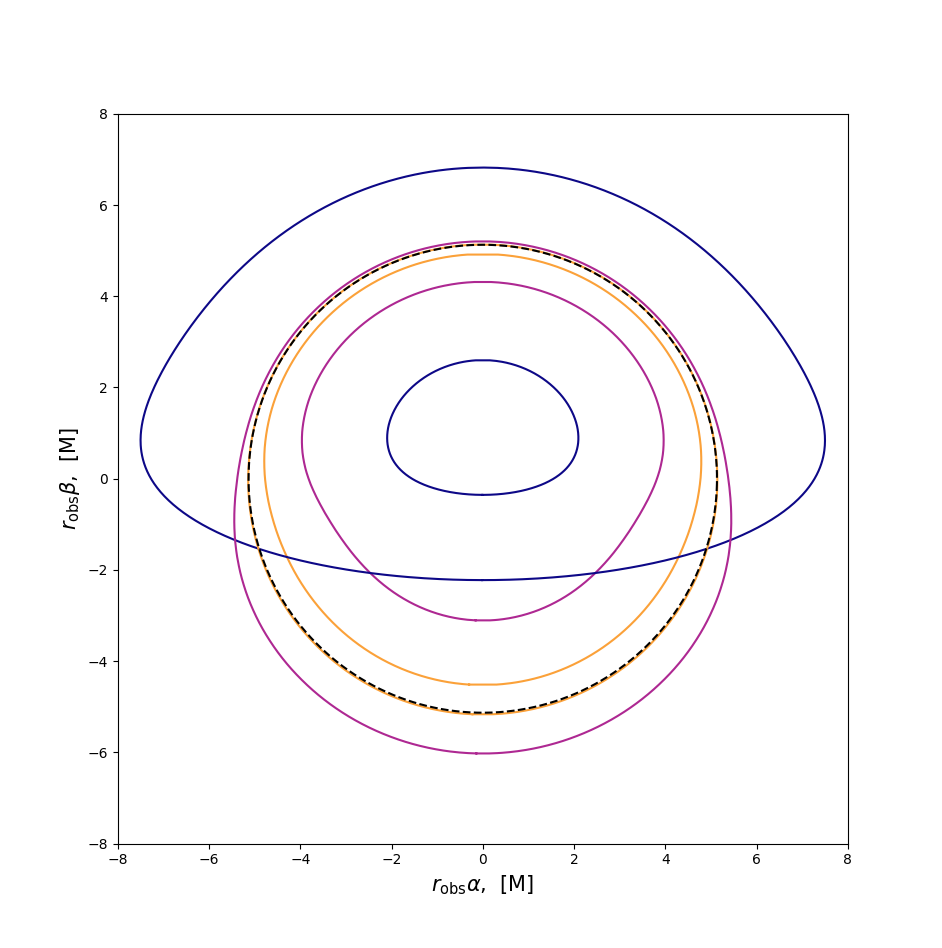
\includegraphics[scale = 0.2]{Section_6_Morphology_of_the images_of_horizonless_spacetimes/WH_70_deg_r6_gamma_2.png}
		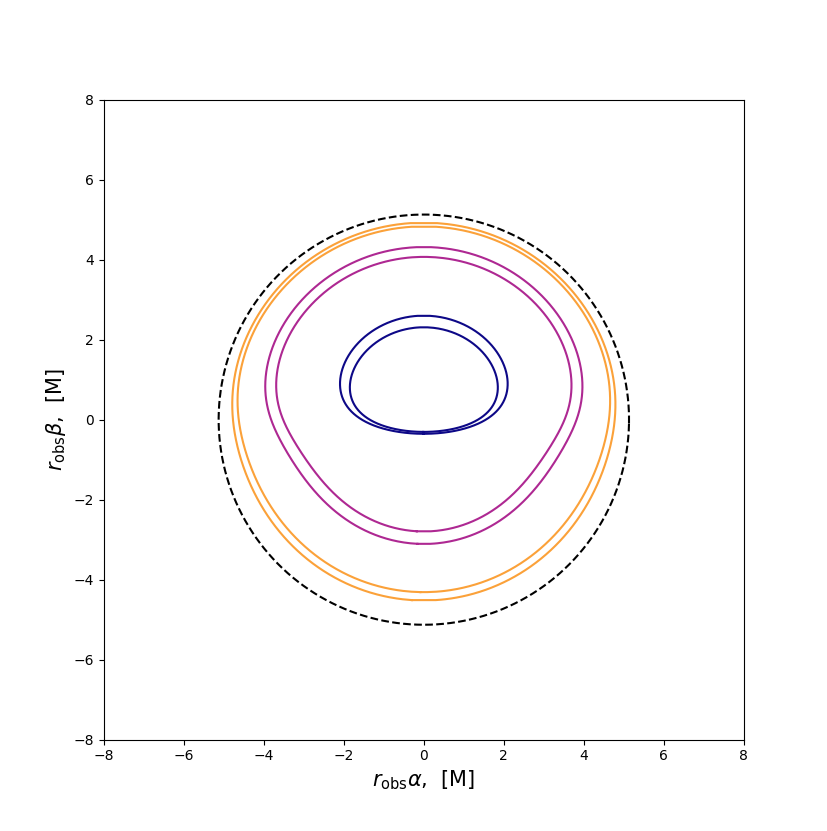
\includegraphics[scale = 0.23]{Section_6_Morphology_of_the images_of_horizonless_spacetimes/WH_70_deg_r6_r500.png}
				
		\tiny V Deliyski, G Gyulchev, P Nedkova, and S Yazadjiev. Observational features
		of thin accretion disks around traversable wormholes. Journal of Physics:
		Conference Series, 2255(1):012002, apr 2022.
		
		
	\end{frame}
	
	\subsection{Наблюдателна релевантност}
	
	\begin{frame}{Наблюдателна релевантност}

		\centering
		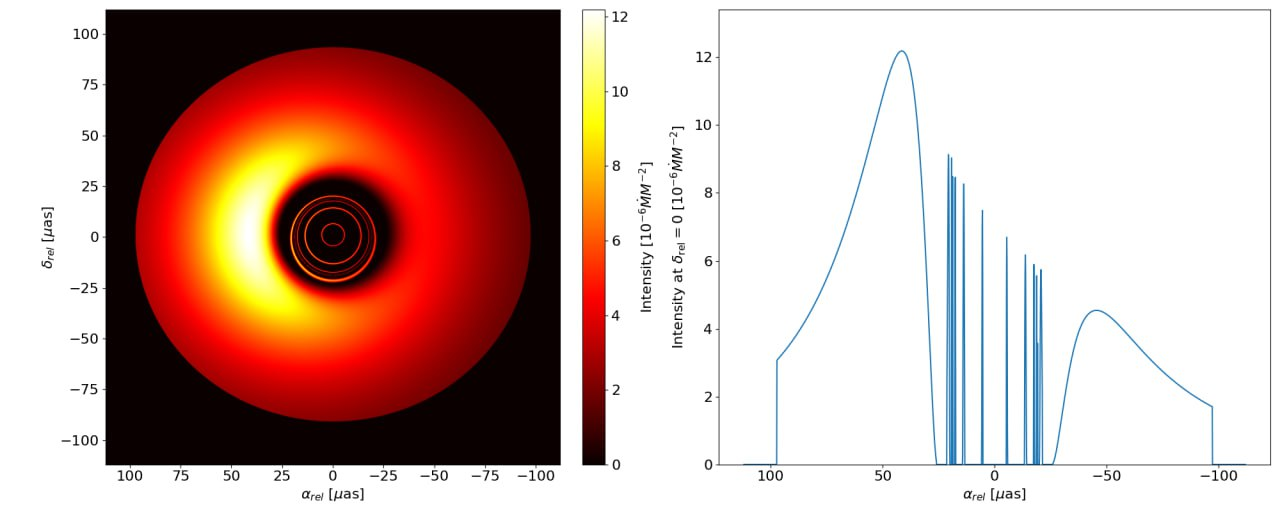
\includegraphics[scale = 0.3]{Pre-Defence/WH_20_deg.jpg}
		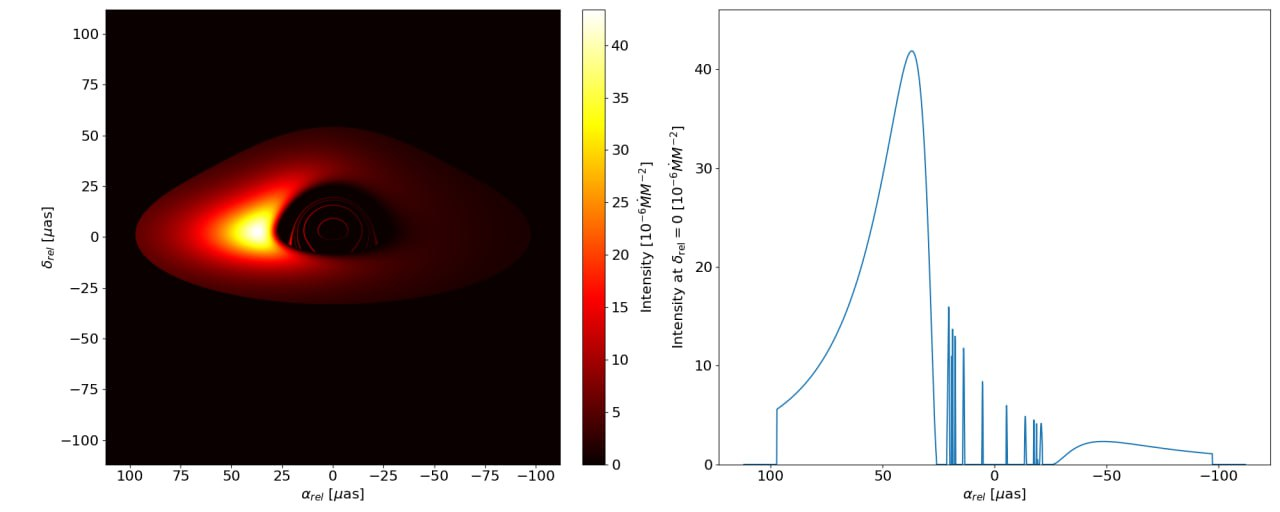
\includegraphics[scale = 0.3]{Pre-Defence/WH_70_deg.jpg}

		
	\end{frame}
	
	\section{Отпечатък на пространство-времето върху поляризацията на образите}
	
	\begin{frame}{Отпечатък на пространство-времето върху поляризацията на образите}
		\begin{block}{Природа да поляризираното лъчение}
			Наблюденията на M87$^*$ и Sgr A$^*$ се описват добре от високо-температурна и оптически тънка плазма, излъчваща синхотронно
		\end{block}
		
		\begin{center}
			$\downarrow$
		\end{center}
		
		\begin{block}{Метод на анализ}
			Използваме опростен модел на излъчващият механизъм, който се възползва от Килинговите симетрии на пространство-времето за да пресметне наблюдаваната на безкрайност поляризация.
		\end{block}
	\end{frame}
	
	\begin{frame}{Поляризационни свойства на екзотични компактни обекти - директни образи}
		\centering
		\centering{\small Пространствено-времеви тунел}
		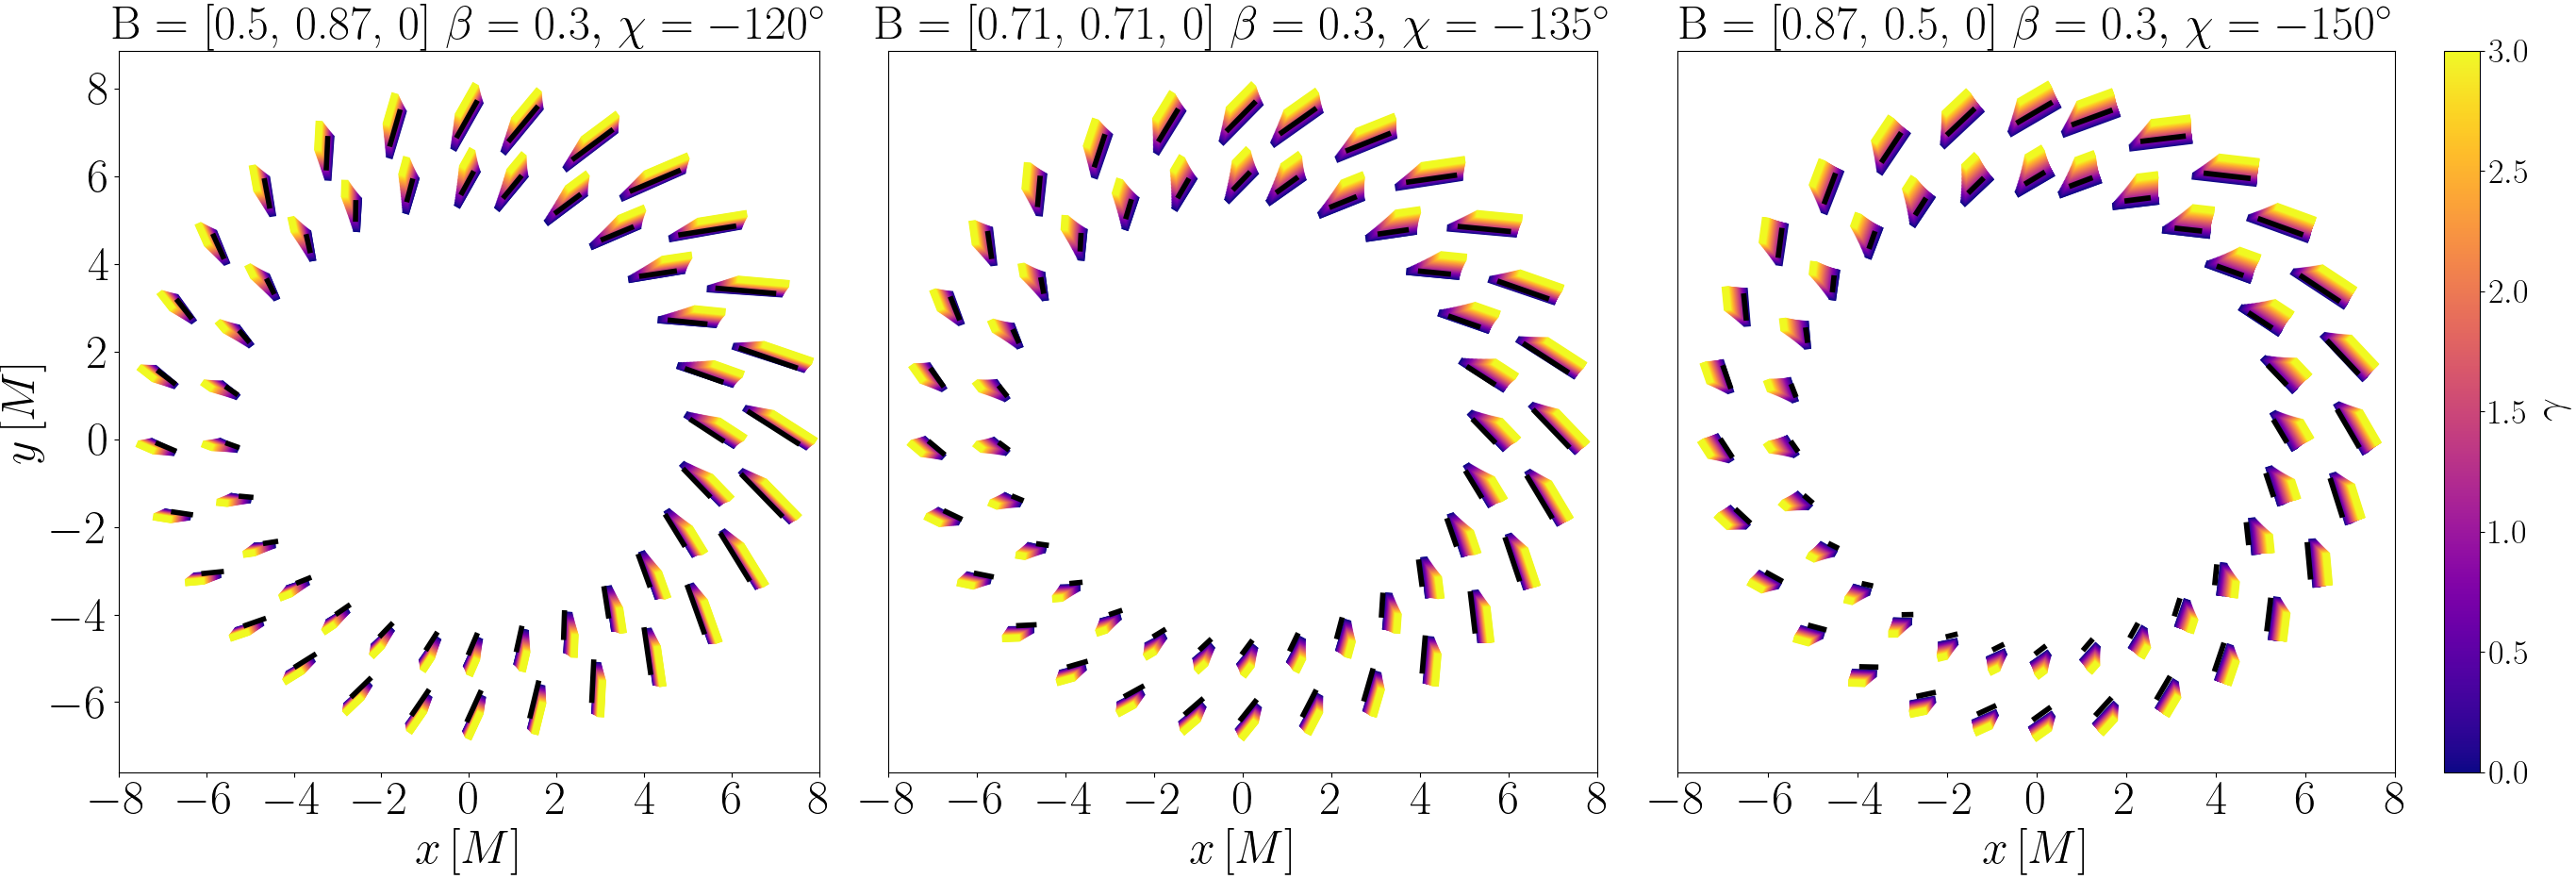
\includegraphics[scale = 0.14]{Section_7_Polarized_Emission/WH_alpha_Eq_Field.png}\\
		\centering{\small Гола сингуларност на Джанис-Нюман-Уиникър}
		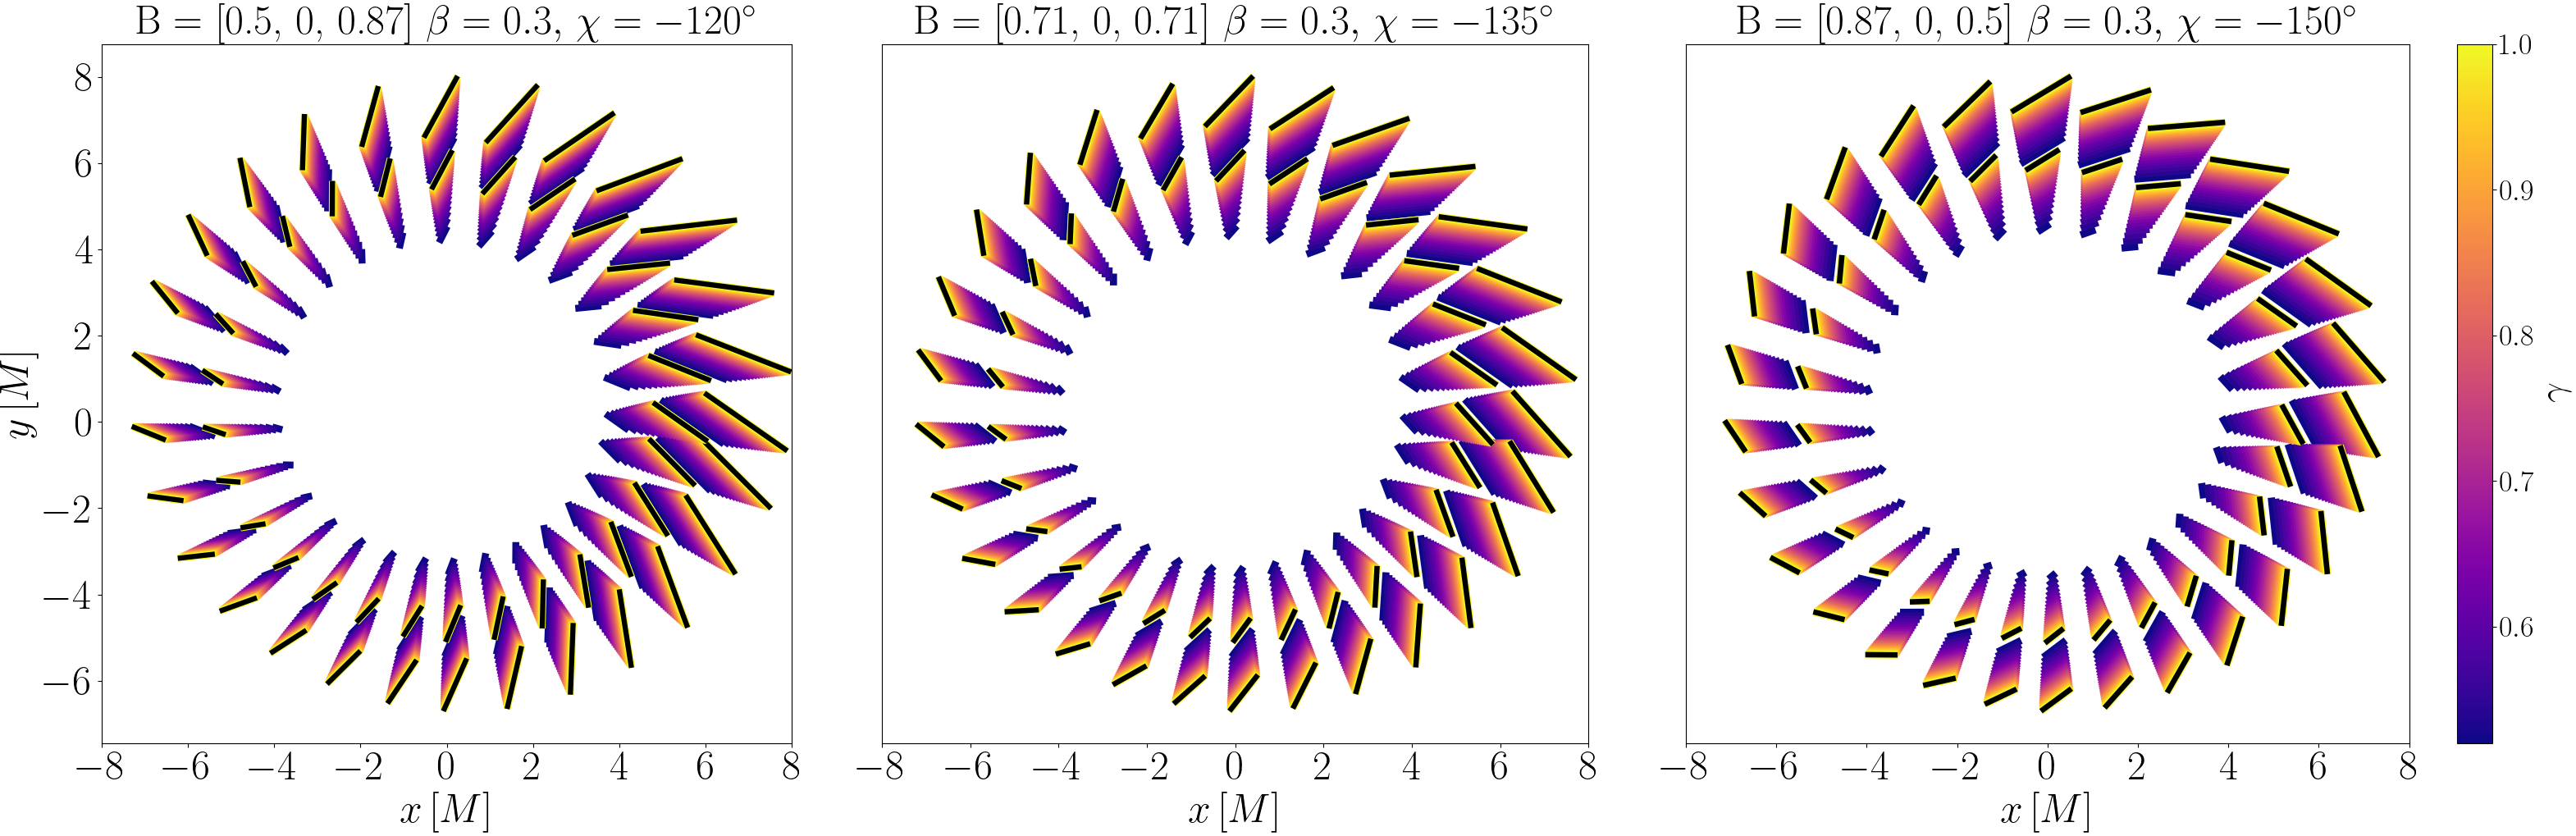
\includegraphics[scale = 0.12]{Section_7_Polarized_Emission/JNW_alpha_Eq_Field.png}
	\end{frame}
	
	\begin{frame}{Поляризационни свойства на екзотични компактни обекти - индиректни образи}
		
		\centering
		\centering{\small Пространствено-времеви тунел}
		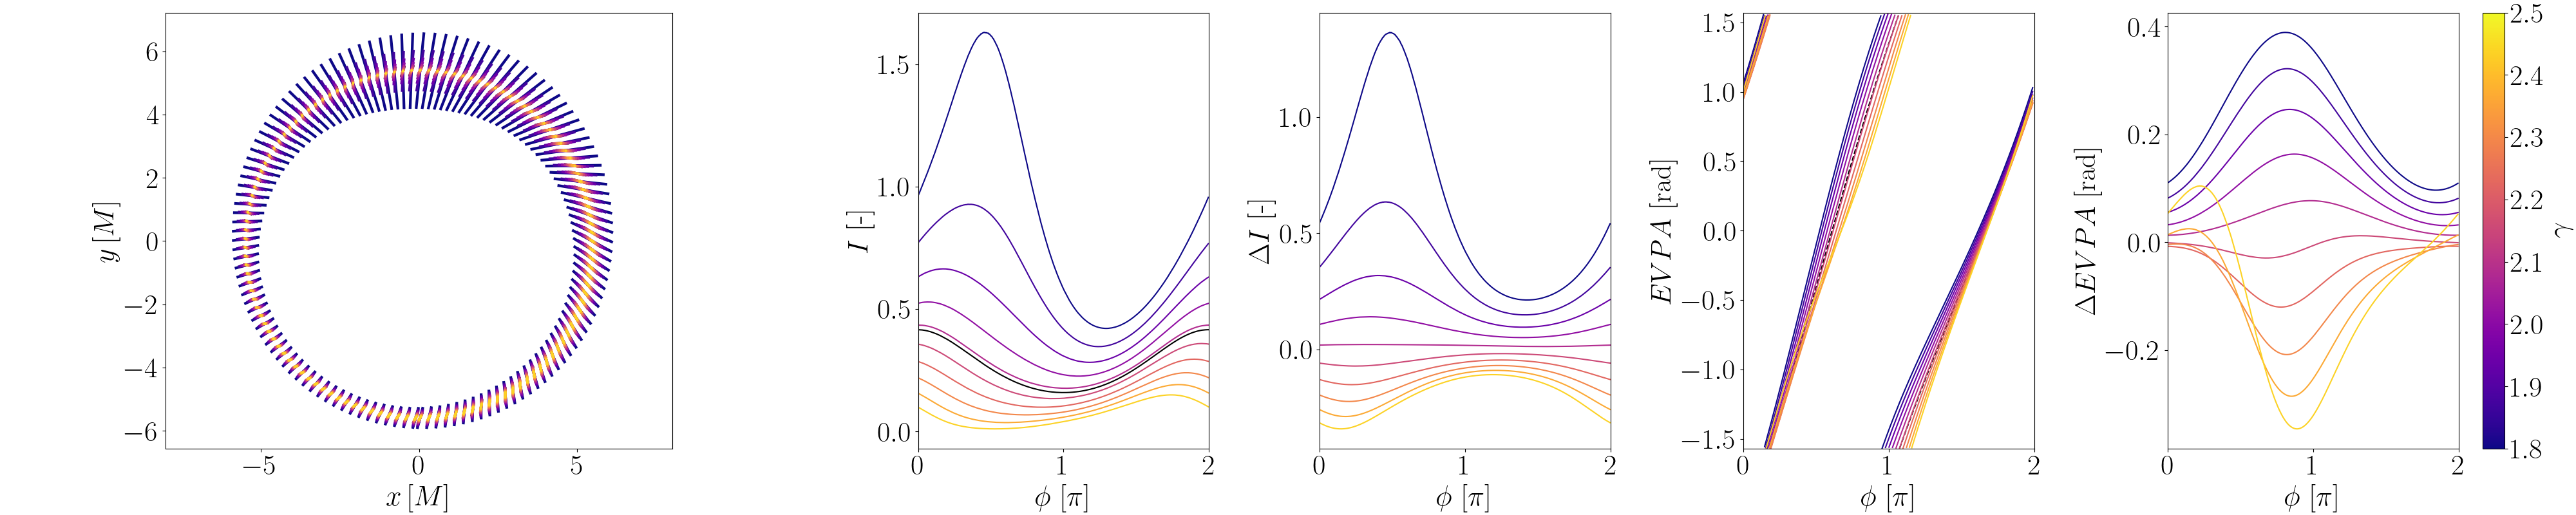
\includegraphics[scale = 0.12]{Section_7_Polarized_Emission/WH_delta_fig_B_0.5_0.87_0_20_deg_r6_n1.png}
		\centering{\small Гола сингуларност на Джанис-Нюман-Уиникър}
		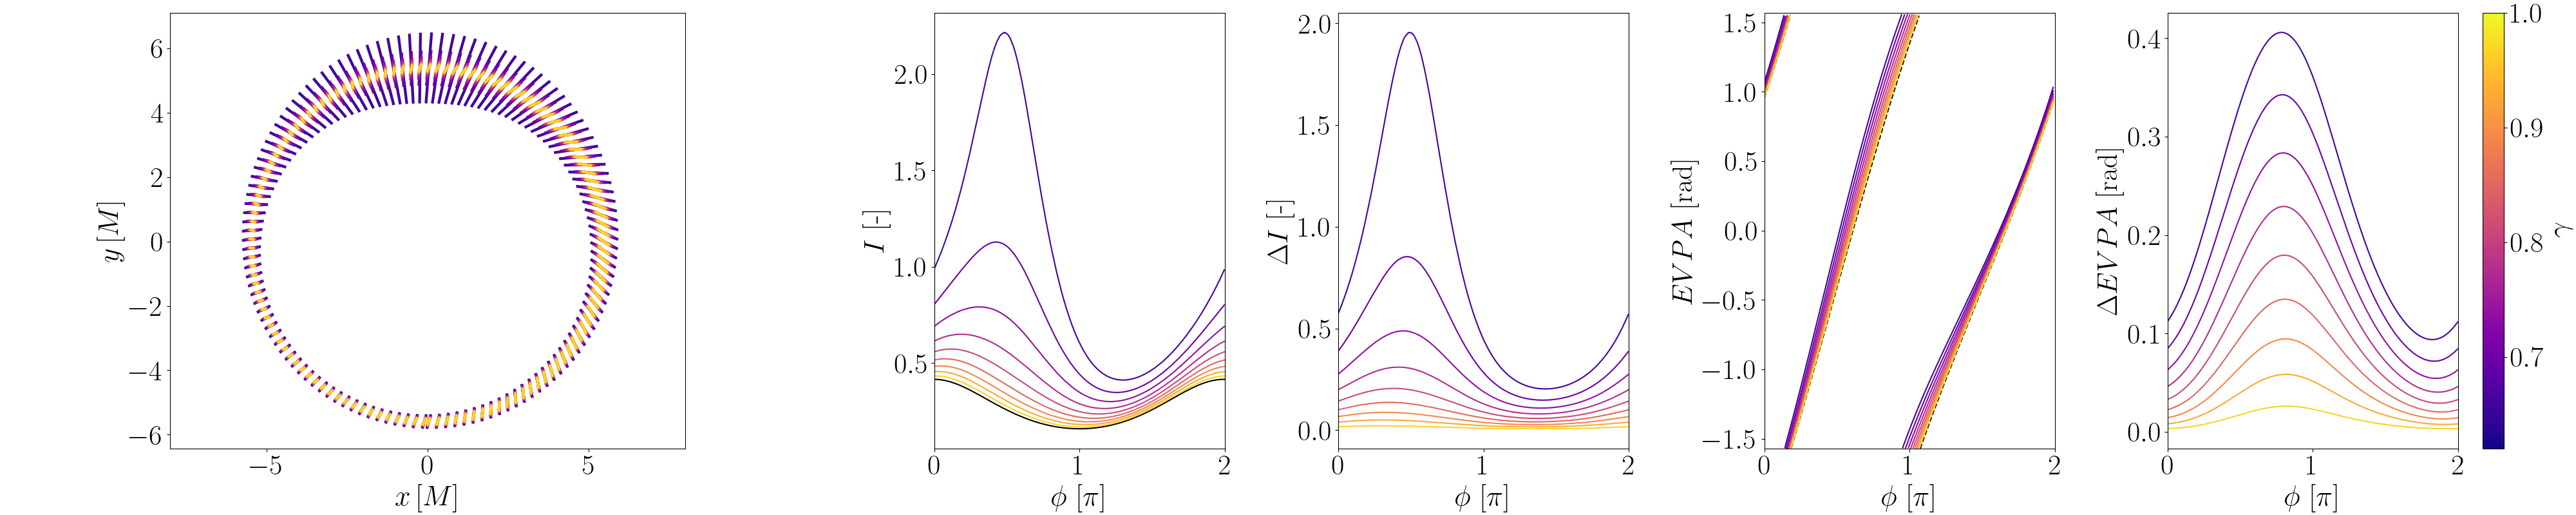
\includegraphics[scale = 0.12]{Section_7_Polarized_Emission/JNW_delta_fig_B_0.5_0.87_0_20_deg_r6_n1.png}\\
		
			
		\tiny  $\bullet$ V Deliyski, G Gyulchev, P Nedkova, and S Yazadjiev.
		Polarized image of equatorial emission in horizonless spacetimes: Traversable
		wormholes. Phys. Rev. D, 106:104024, Nov 2022.\\
		$\bullet$ V Deliyski, G Gyulchev, P Nedkova, and S Yazadjiev.
		Polarized image of equatorial emission in horizonless spacetimes: Naked
		singularities. Phys. Rev. D, 108:104049, Nov 2023.
		
	\end{frame}

	
	\section{Наблюдения на екзотични компактни обекти от ngEHT}
	
	\subsection{VLBI наблюдения}
	
	\begin{frame}{VLBI наблюдения}

		\centering
		\qquad
		\begin{minipage}{11em}
			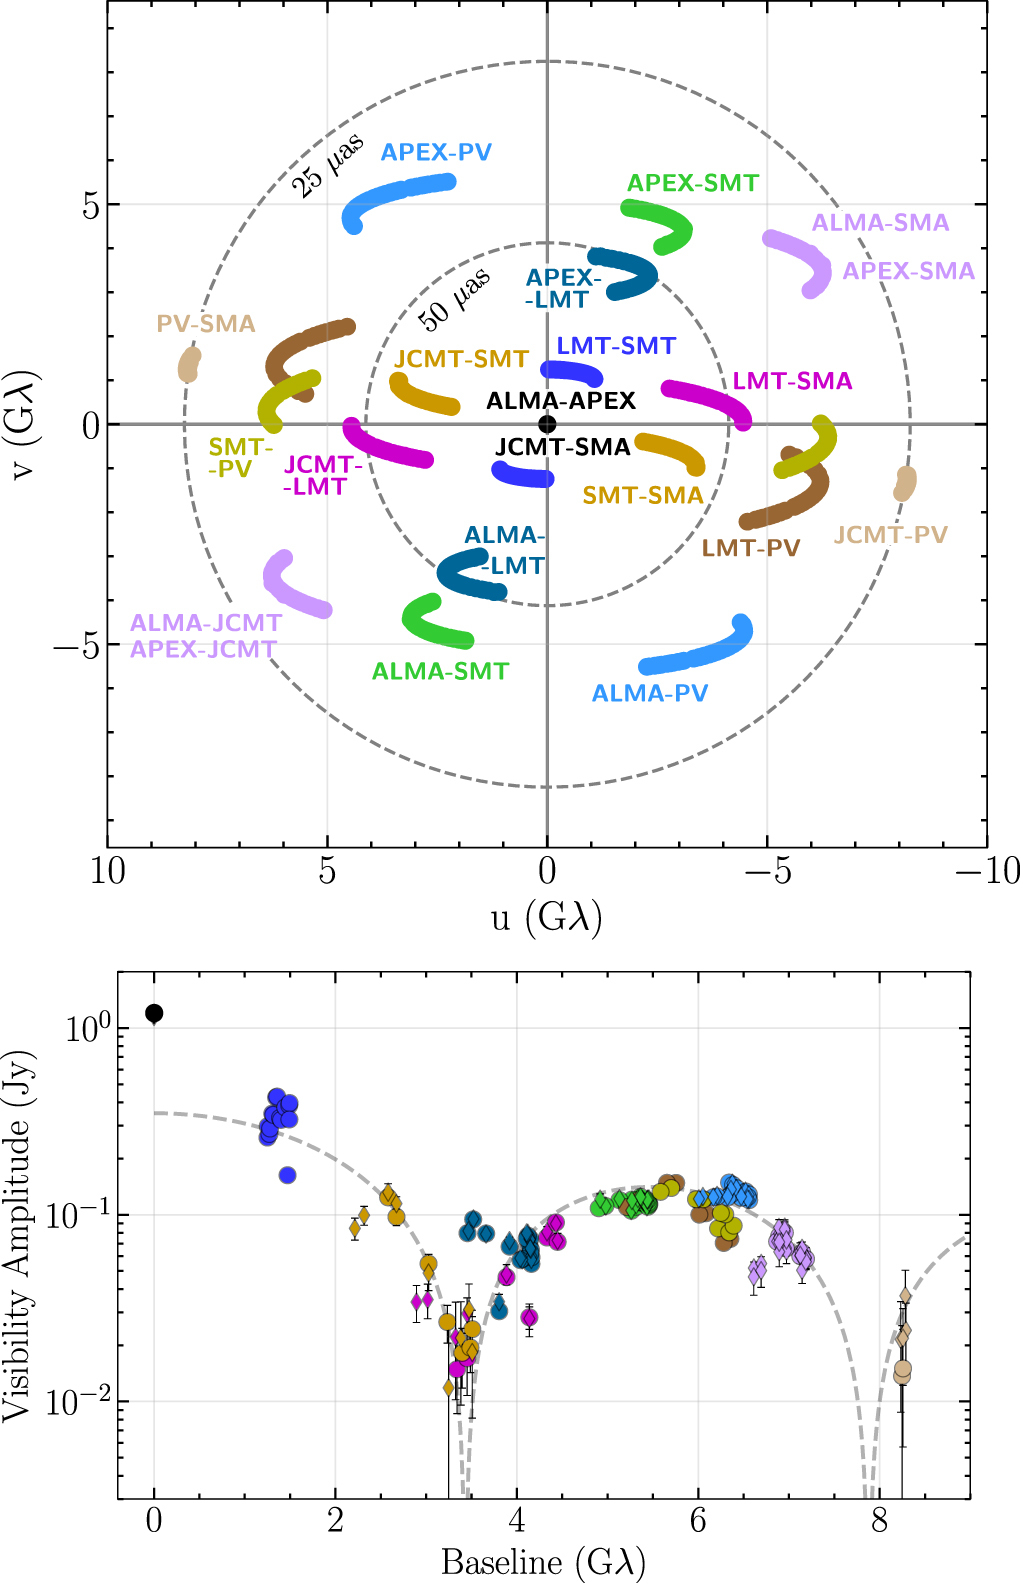
\includegraphics[scale = 0.5]{Pre-Defence/UV_coverage.jpg}
		\end{minipage}\,\,\,\huge$\rightarrow$
		\begin{minipage}{8em}
			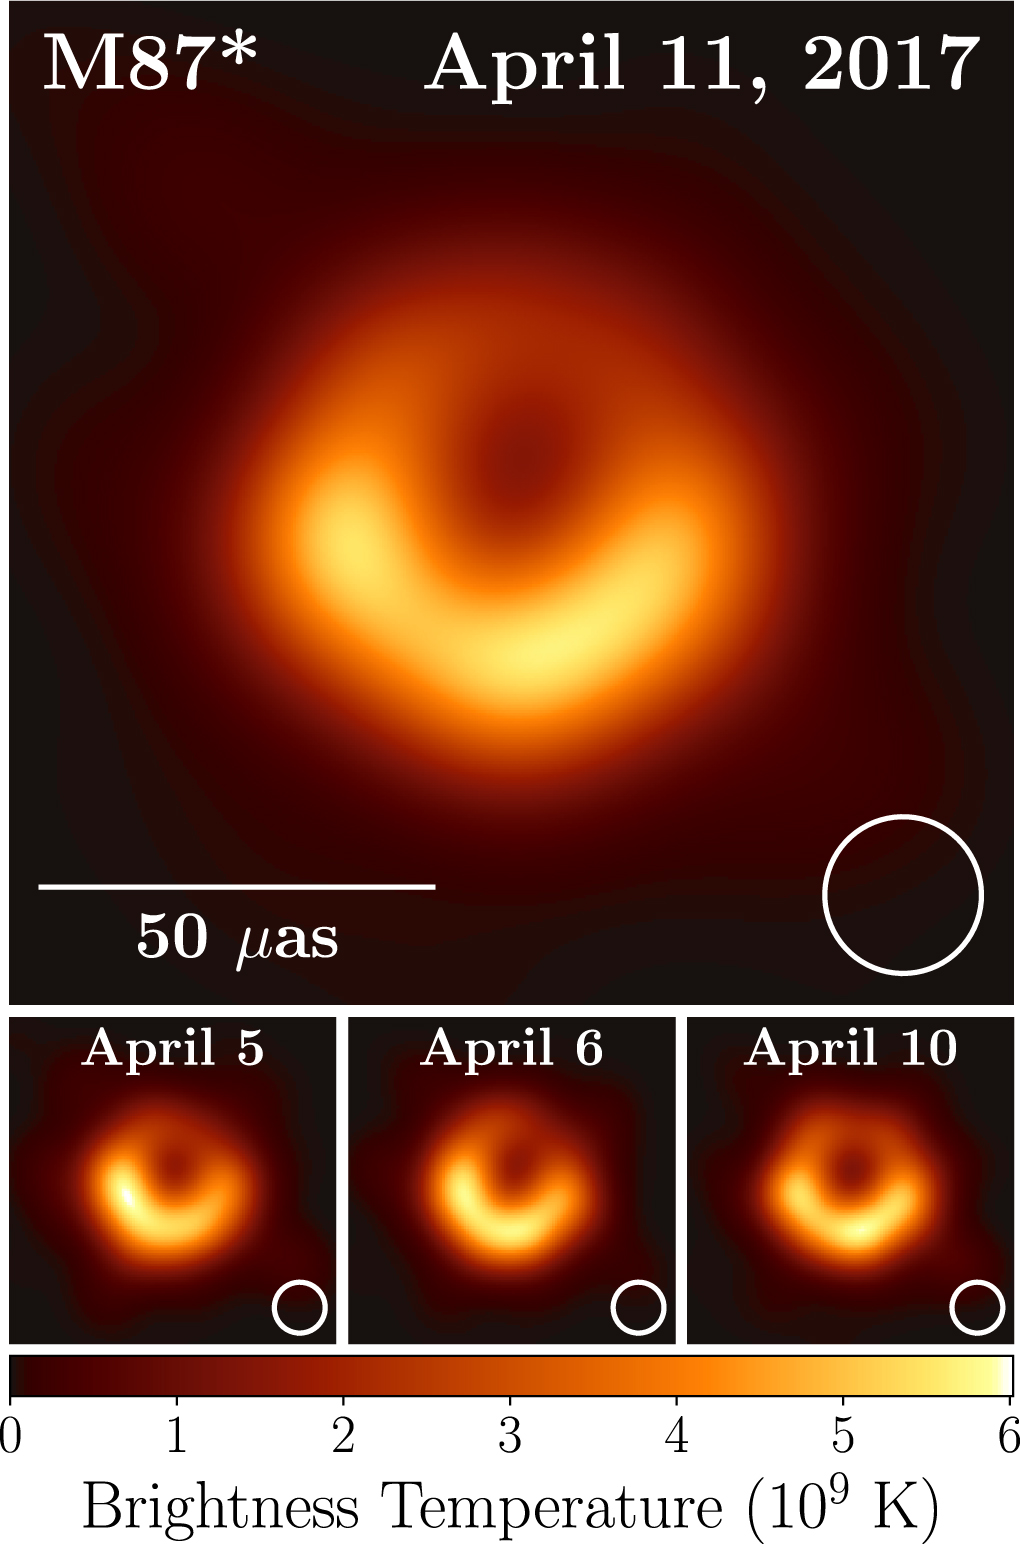
\includegraphics[scale = 0.5]{Pre-Defence/M87.jpg}
		\end{minipage}\\
		
		\tiny The Event Horizon Telescope Collaboration et al 2019 ApJL 875 L1
		
	\end{frame}
	
	\subsection{Методика за симулиране на VLBI наблюдения}
	
	\begin{frame}{Методика за симулиране на VLBI наблюдения}
		
		\begin{block}{Генериране на "идеално"$\,$ наблюдение}
			\small
			\begin{subequations}
				\begin{equation*}
					\frac{dx^\mu}{d\lambda} = \frac{\partial H}{\partial k_\mu},\quad \frac{d k_\mu}{d\lambda} = - \frac{\partial H}{\partial x^\mu},\quad 
					k^\nu\nabla_\nu f^\mu = 0
				\end{equation*}
				\begin{equation*}
					\frac{d}{d\lambda} \begin{pmatrix}
						\mathcal{I}_\nu\\
						\mathcal{Q}_\nu\\
						\mathcal{U}_\nu\\
						\mathcal{V}_\nu
					\end{pmatrix} = 
					\begin{pmatrix}
						\mathcal{J}_\mathcal{I,\nu}\\
						\mathcal{J}_\mathcal{Q,\nu}\\
						\mathcal{J}_\mathcal{U,\nu}\\
						\mathcal{J}_\mathcal{V,\nu}
					\end{pmatrix}
					-	\begin{pmatrix}
						\kappa_\mathcal{I,\nu} & \kappa_\mathcal{Q,\nu} & \kappa_\mathcal{U,\nu} & \kappa_\mathcal{V,\nu}\\
						\kappa_\mathcal{Q,\nu}& \kappa_\mathcal{I,\nu}& -\rho_\mathcal{U,\nu}& \rho_\mathcal{V,\nu}\\     	
						\kappa_\mathcal{U,\nu}& -\rho_\mathcal{V,\nu}& \kappa_\mathcal{I,\nu}& \rho_\mathcal{Q,\nu}\\	  
						\kappa_\mathcal{V,\nu}& \rho_\mathcal{U,\nu}& -\rho_\mathcal{Q,\nu}& \kappa_\mathcal{I,\nu}\\
					\end{pmatrix}
					\begin{pmatrix}
						\mathcal{I}_\nu\\
						\mathcal{Q}_\nu\\
						\mathcal{U}_\nu\\
						\mathcal{V}_\nu
					\end{pmatrix}
				\end{equation*}
			\end{subequations}
			
		\end{block}
		
		\centering
		\includegraphics[scale = 0.5]{Pre-Defence/github.png}
		\small https://github.com/ValentinDeliyski/Mjolnir\_GRRT/tree/develop
	\end{frame}
	
	\begin{frame}{Генериране на "идеално"$\,$ наблюдение}
		\centering
		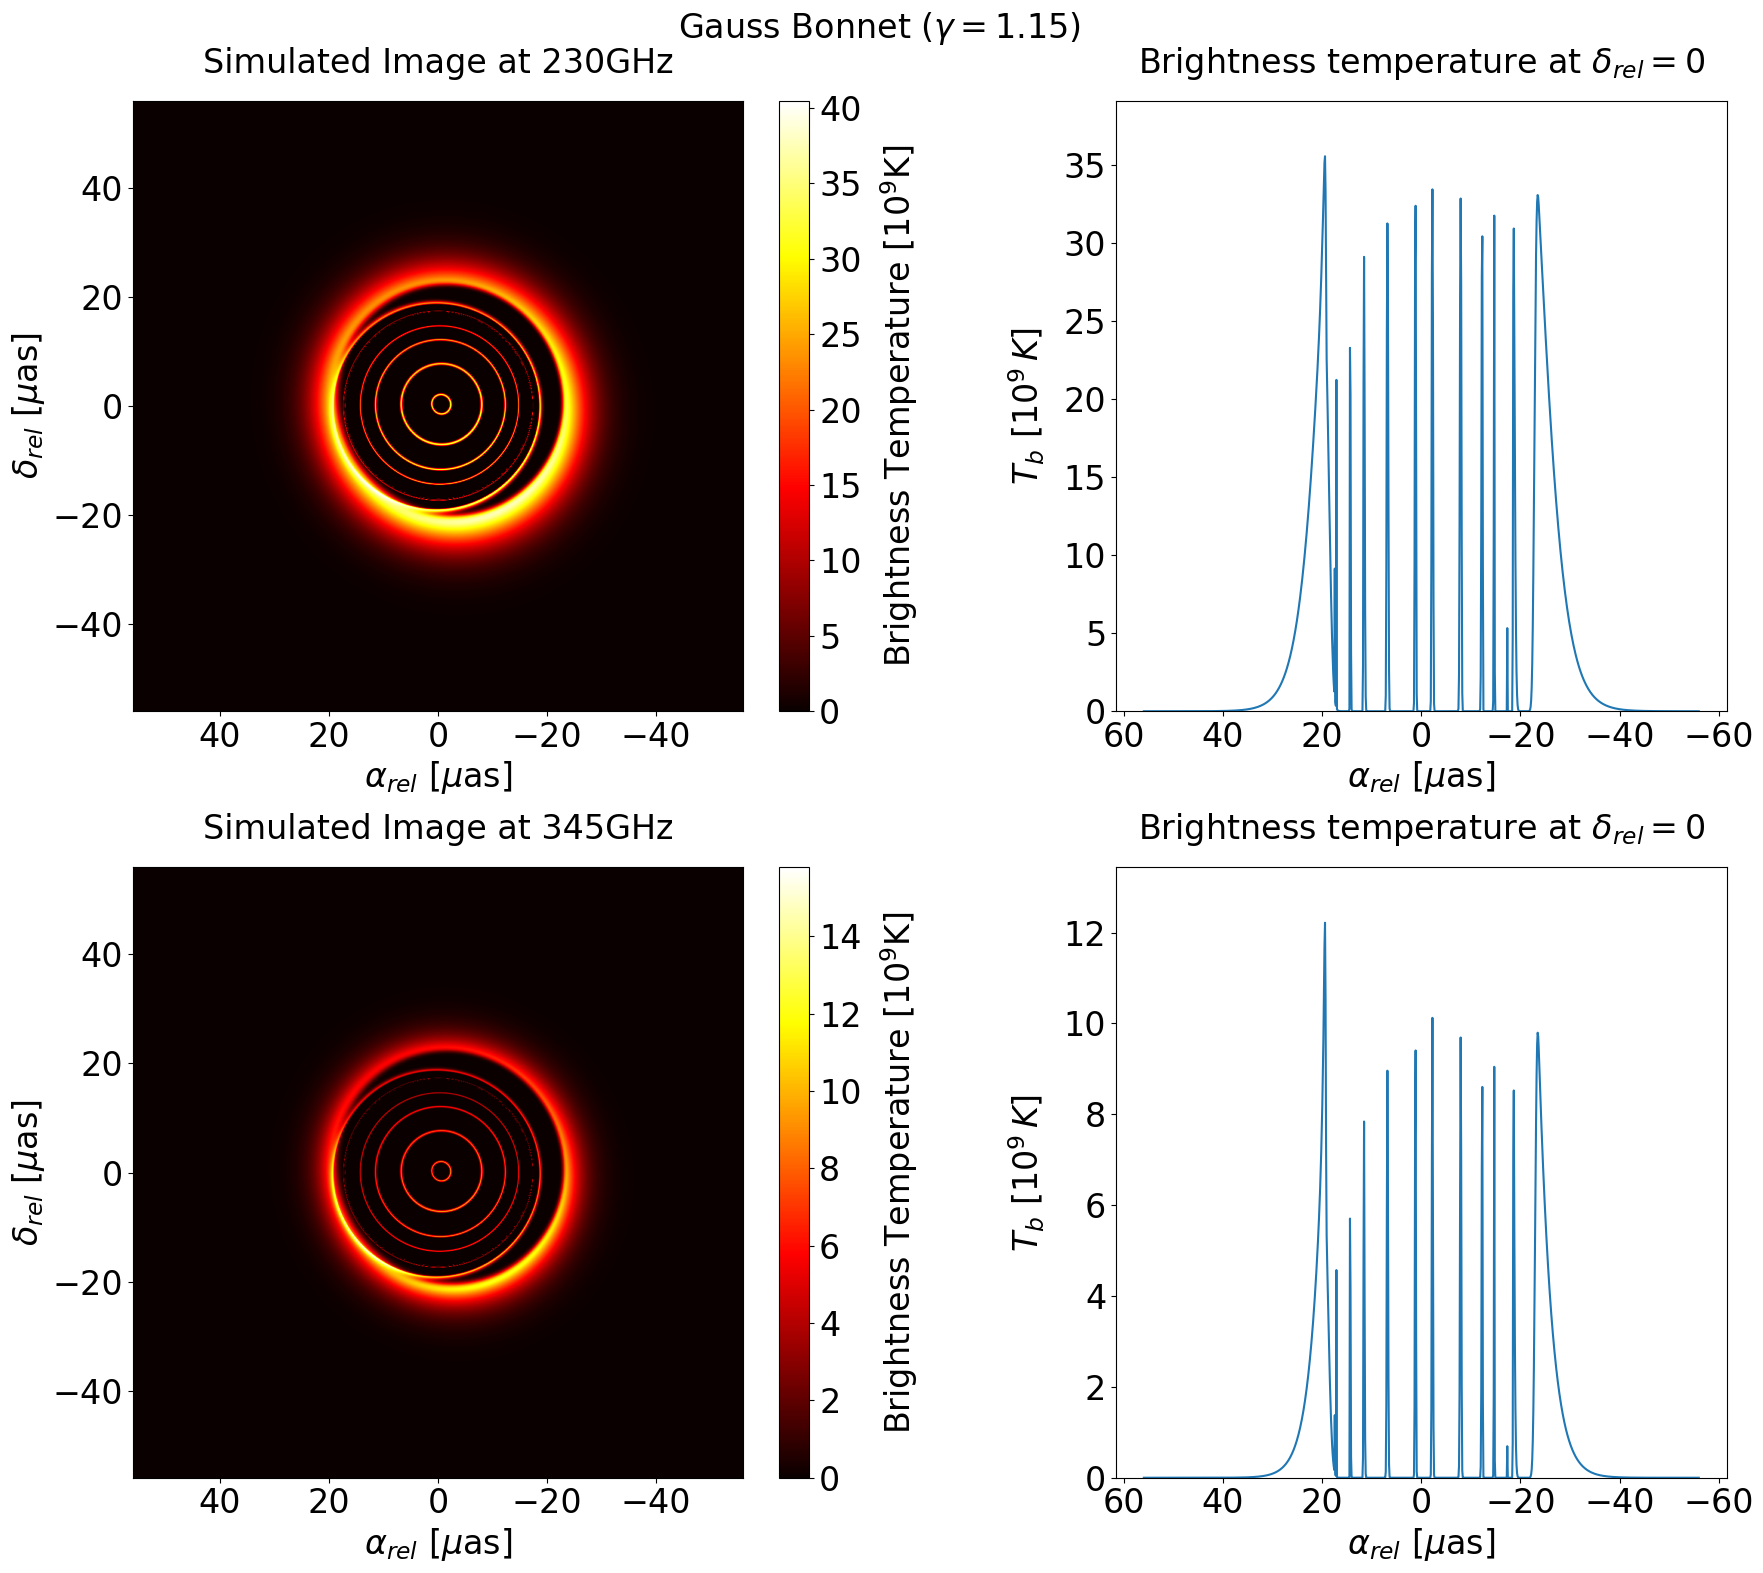
\includegraphics[scale = 0.18]{Pre-Defence/Ray_tracer_plot_230_345.png}\\
		
		\tiny V Deliyski, G Gyulchev, P Nedkova, and S Yazadjiev.
		Observing naked singularities by the present and next-generation event horizon
		telescope. http://arxiv.org/abs/2401.14092, 2024.
	\end{frame}
	
	\begin{frame}{Генериране на реално наблюдение с пакета \textbf{ehtim}}
			\centering
		\begin{minipage}{13em}
			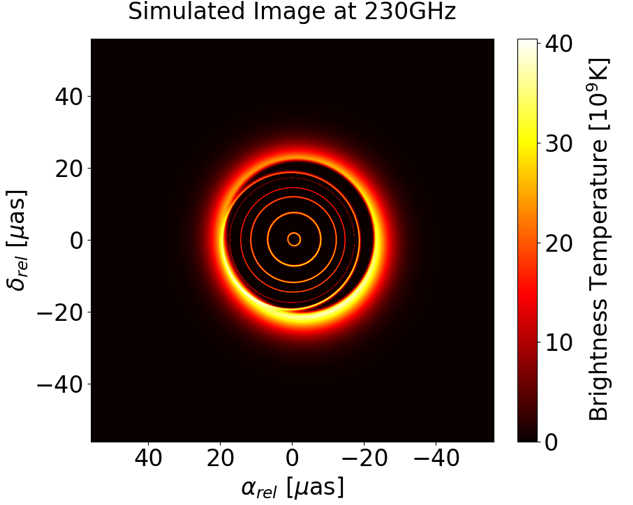
\includegraphics[scale = 0.50]{Pre-Defence/GB_ray_tracer_230.png}
		\end{minipage}\qquad$\rightarrow$
		\begin{minipage}{13em}
			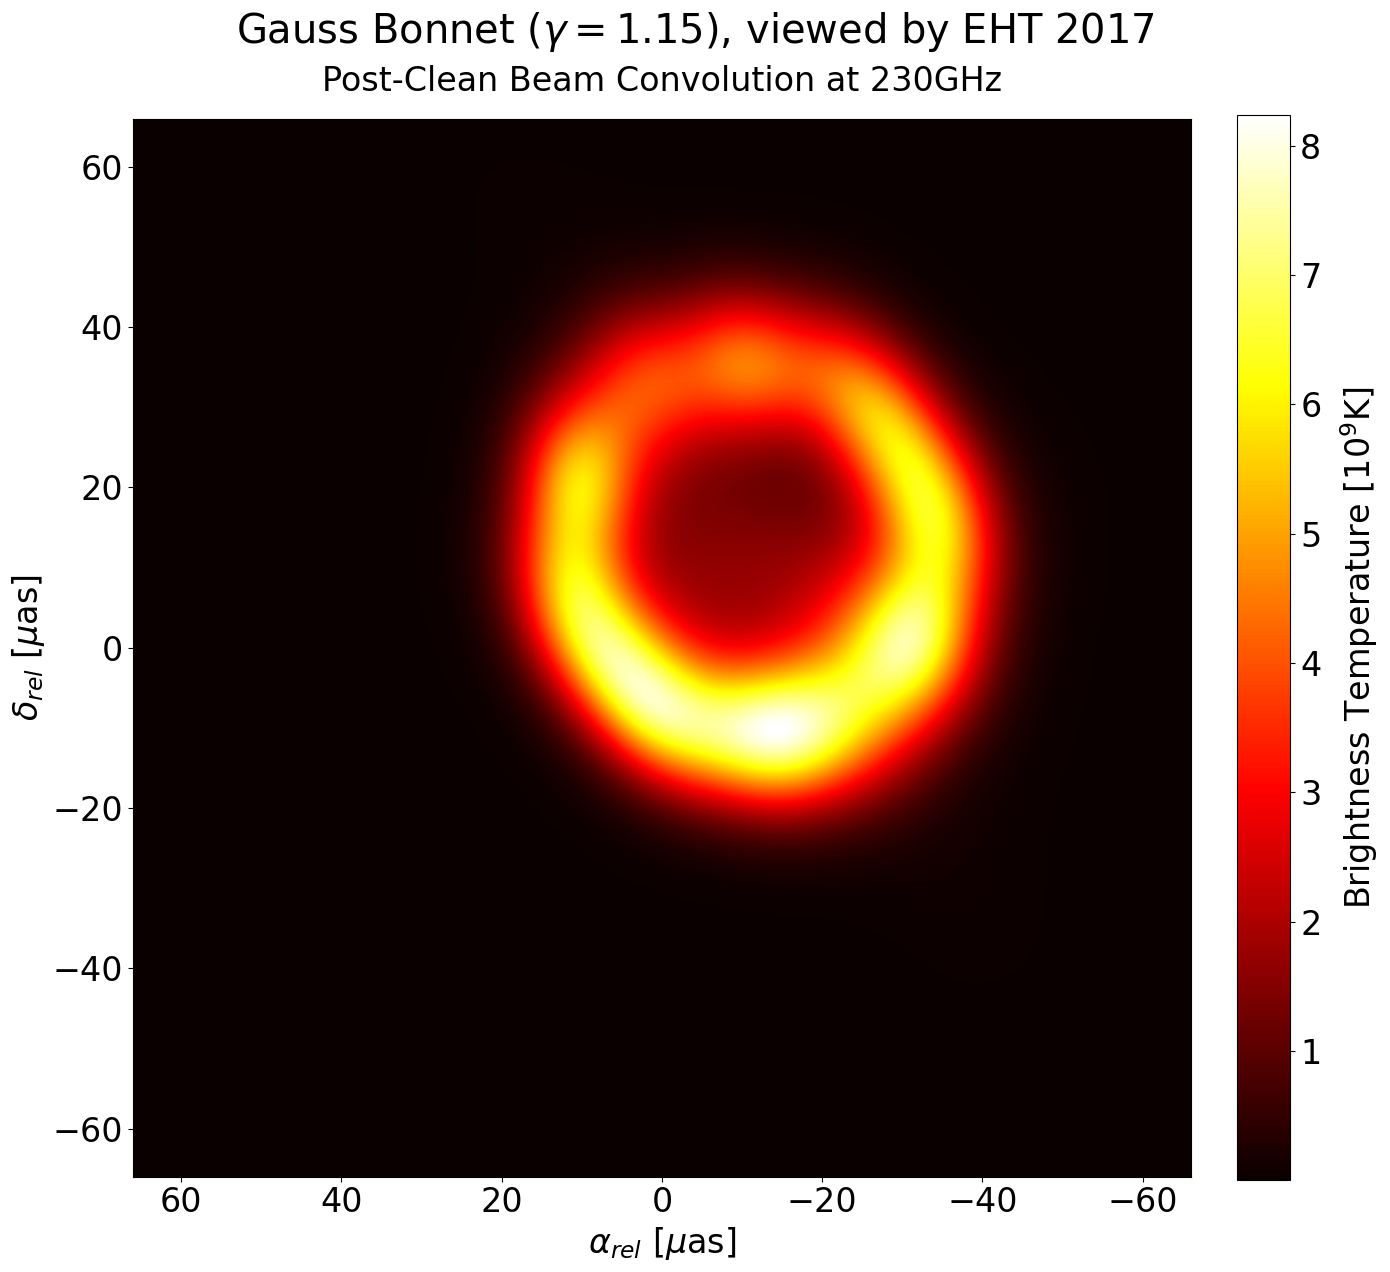
\includegraphics[scale = 0.14]{Pre-Defence/Ehtim_plot_2017.png}
		\end{minipage}\\
		
		\tiny V Deliyski, G Gyulchev, P Nedkova, and S Yazadjiev.
		Observing naked singularities by the present and next-generation event horizon
		telescope. http://arxiv.org/abs/2401.14092, 2024.
		\centering
		
\includegraphics[scale = 0.5]{Pre-Defence/ehtim_github.png}
		\small https://github.com/achael/eht-imaging
	\end{frame}
	
	\begin{frame}{Генериране на реално наблюдение с пакета \textbf{ehtim}}
		\centering
		\begin{minipage}{13em}
			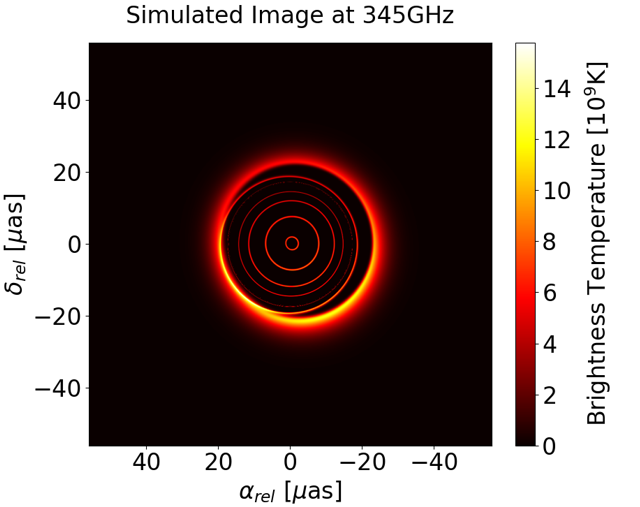
\includegraphics[scale = 0.50]{Pre-Defence/GB_ray_tracer_345.png}
		\end{minipage}\qquad$\rightarrow$
		\begin{minipage}{13em}
			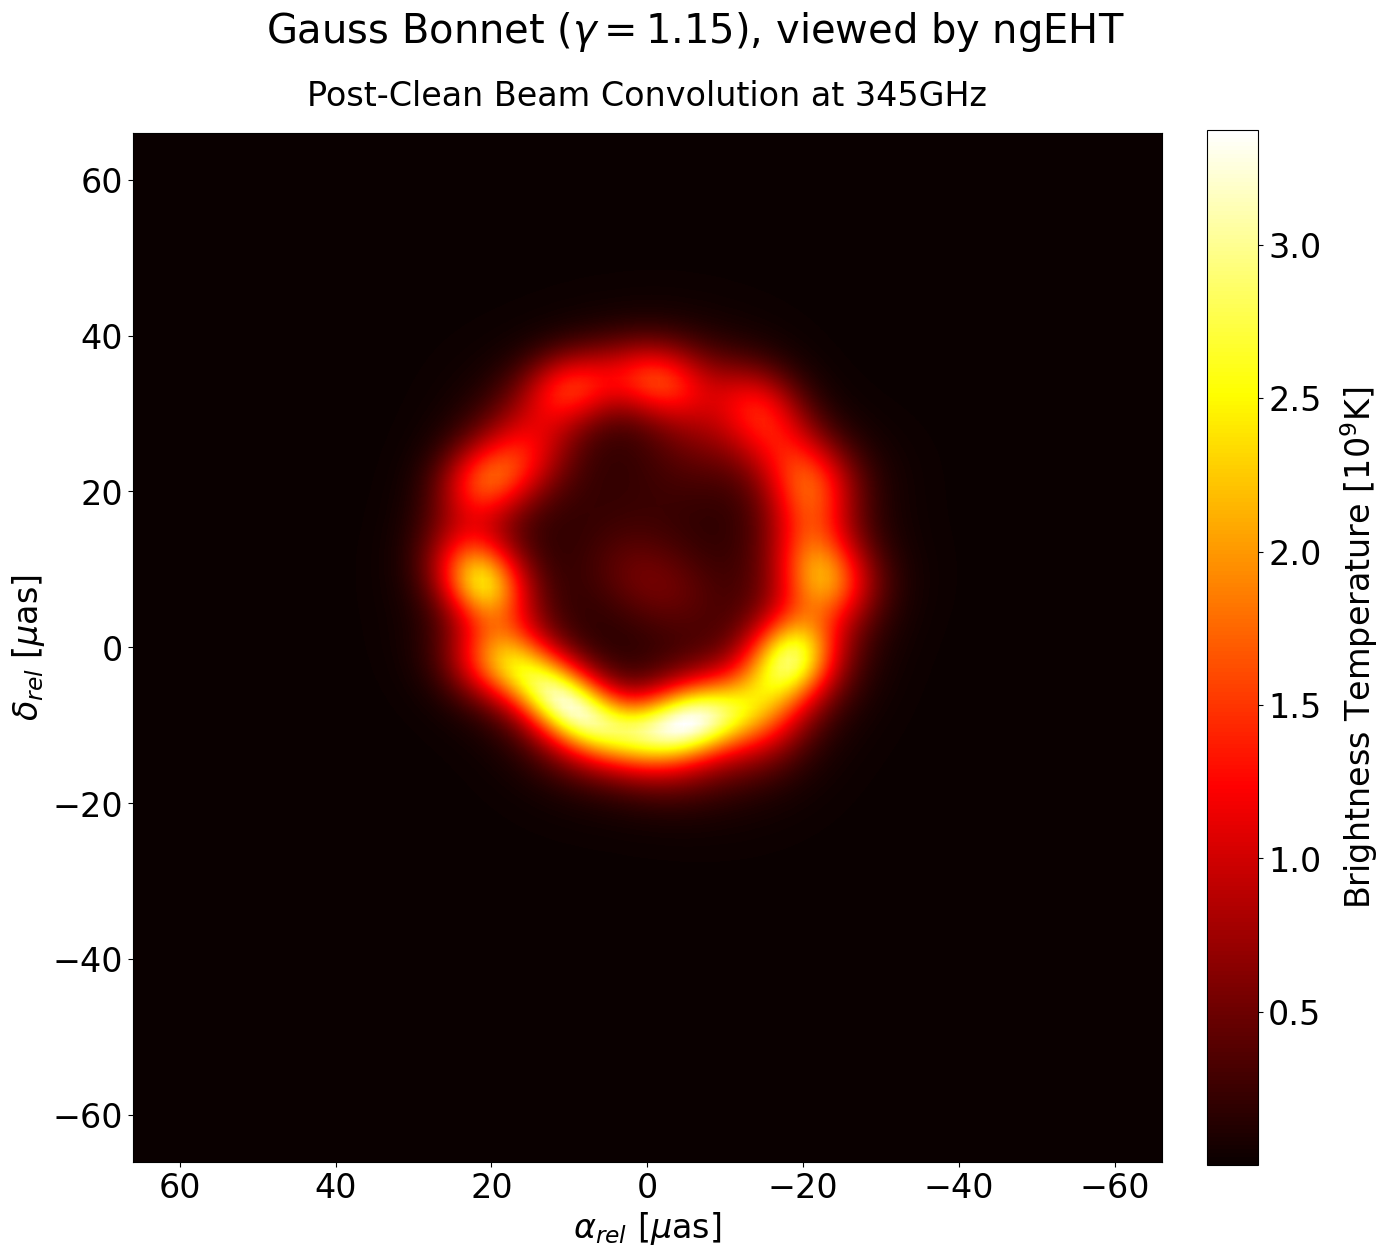
\includegraphics[scale = 0.14]{Pre-Defence/Ehtim_plot_ngEHT_345.png}
		\end{minipage}\\
		
		\tiny V Deliyski, G Gyulchev, P Nedkova, and S Yazadjiev.
		Observing naked singularities by the present and next-generation event horizon
		telescope. http://arxiv.org/abs/2401.14092, 2024.
	\end{frame}
	
	\begin{frame}{Морфологичен анализ на образите с пакета \textbf{VIDA}}

		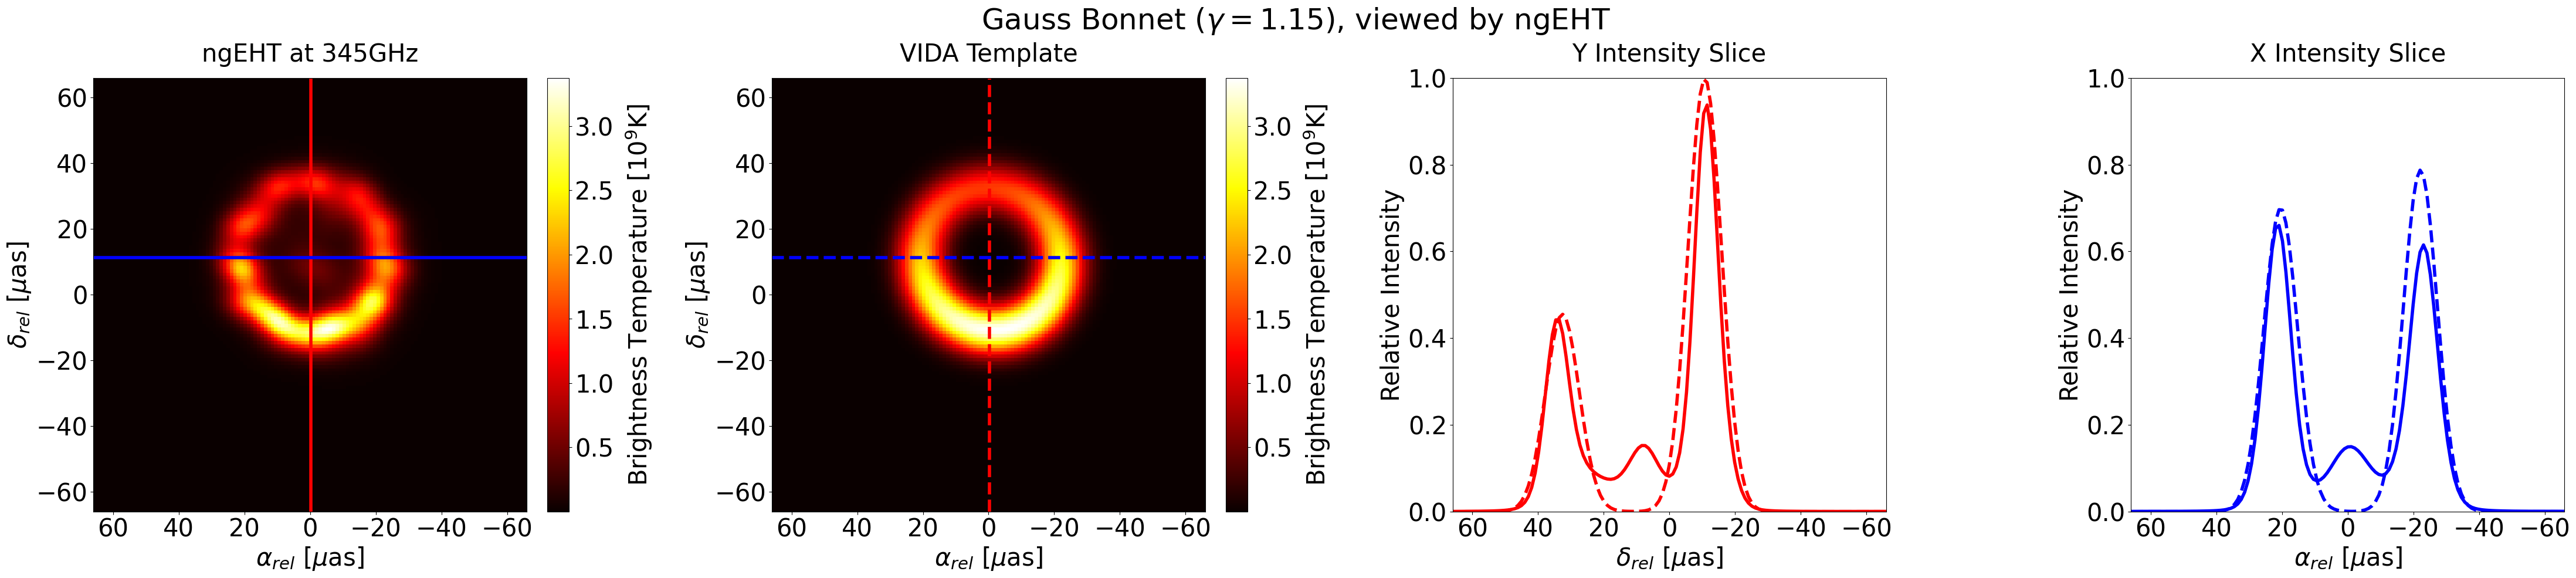
\includegraphics[scale = 0.11]{Pre-Defence/Ehtim_Vida_plot_ngEHT_345.png}\\
		
		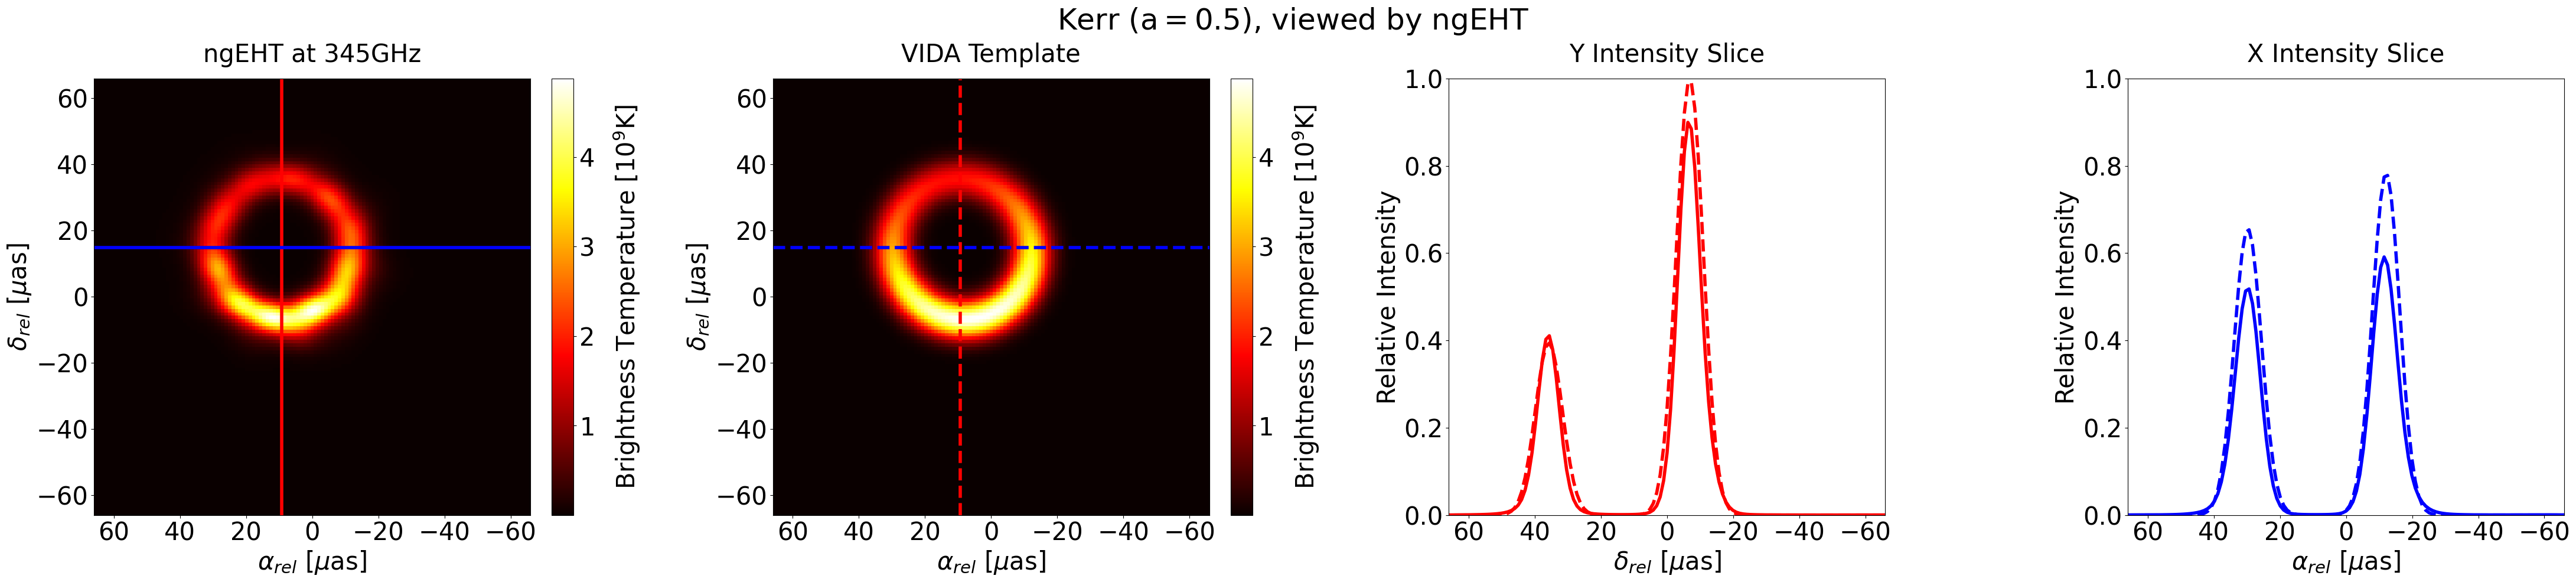
\includegraphics[scale = 0.11]{Pre-Defence/Ehtim_Vida_plot_ngEHT_345_kerr.png}\newline
		\tiny V Deliyski, G Gyulchev, P Nedkova, and S Yazadjiev.
		Observing naked singularities by the present and next-generation event horizon
		telescope. http://arxiv.org/abs/2401.14092, 2024.\\
		
		\small
		Количествена оценка за морфологията даваме с $f_c = \frac{\min\mathcal{F}_{\text{center}}}{\langle{\mathcal{F}}_{\text{ring}}\rangle}$\\
		При 230 GHz $f_{c,\text{Kerr}} \approx 10^{-2} - 10^{-3}$, $f_{c,\text{GB}} > 10^{-1} $\\
		
		\centering \small https://github.com/ptiede/VIDA.jl
	\end{frame}
	
	\begin{frame}
		\centering
		Благодаря!
	\end{frame}
	
\end{document}